\section{Interrupts}
\subsection{Interrupt-Klassen}
\begin{itemize}
    \item Hardware-Fehler
    \item Timer
    \item I/O
    \item Software-Interrupts
    \begin{itemize}
        \item Arithmetik
        \item Traps
        \item etc.
    \end{itemize}
\end{itemize}

\subsection{Ablauf}
\begin{enumerate}
    \item Interrupt
    \item Kontext-Wechsel
    \item Interrupt-Vector
    \item Interrupt-Handler
    \item Scheduler
\end{enumerate}

\subsection{Round Robin: I/O- vs CPU-lastig}
\textbf{CPU-lastinge} Prozesse nutzen ihre \textbf{Zeitquanten} vollständig, während \textbf{I/O}
Prozesse \textbf{warten} müssen.

\subsection{Interrupt Handling}
\begin{figure}[ht!]
    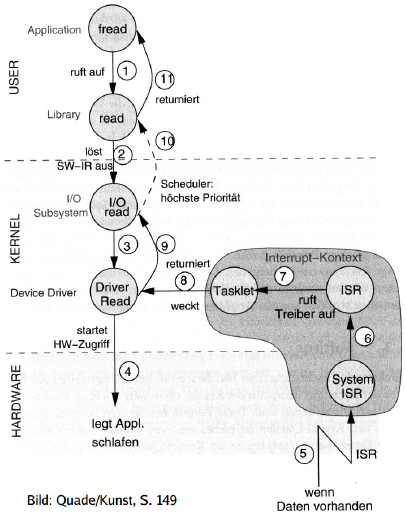
\includegraphics[scale=.8]{pics/isr}
    \caption{Interrupt callgraph}
\end{figure}